\section{Przebieg pracy}
Koordynacja pracy pomiędzy zespołami modułowymi odbywała się głównie przy pomocy GitHub'a. Jest to darmowe, internetowe środowisko do zarządzania współdzielonym kodem oparty o najpopularniejszy system kontroli wersji - Git. Jednym z jego zalet jest możliwość wygenerowania prostych raportów statystycznych. Wykorzstano to do narysowania wykresu przedstawiającego liczbę zmian wysyłanych do głównego repozytorium w czasie (rysunek~\ref{fig:commits}). Pierwsze fragmenty kodu zaczęły pojawiać się w listopadzie. Grudzień i początek stycznia to dalsze, powolne, prace nad aplikacją. Najwięcej zmian pojawiło się w repozytorium pod koniec stycznia i w pierwszych dniach lutego.
\begin{figure}[h]
\centering
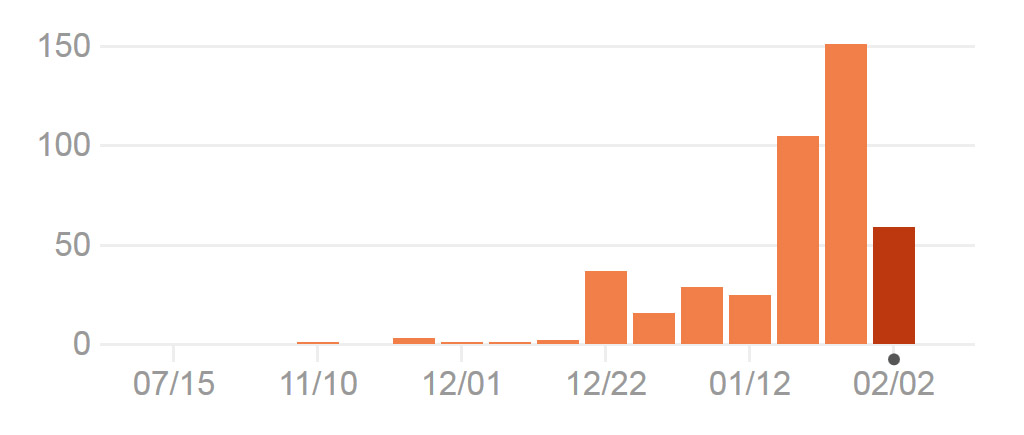
\includegraphics[scale=0.35]{PODSUMOWANIE/commits.jpg}
\caption{Liczba commitów w czasie.}
\label{fig:commits}
\end{figure}